% Dieser Text ist urheberrechtlich gesch�tzt
% Er stellt einen Auszug eines von mir erstellten Referates dar
% und darf nicht gewerblich genutzt werden
% die private bzw. Studiums bezogen Nutzung ist frei
% Mai. 2007
% Autor: Sascha Frank 
% Universit�t Freiburg 
% www.informatik.uni-freiburg.de/~frank/
\documentclass{beamer}
\usepackage{pst-bar,pst-plot,pstricks-add}
\usepackage{graphics,graphicx}
\usepackage{pstricks,pst-node,pst-tree}

\setbeamertemplate{navigation symbols}{}
\beamersetuncovermixins{\opaqueness<1>{25}}{\opaqueness<2->{15}}
\usetheme{CambridgeUS}
\usecolortheme{whale}

\begin{document}
\title{The max-min-hill-climbing algorithm}  
\author[M. Bauer]{Michael Bauer}
\institute[M.Sc. Comp. Science]{M.Sc. Comp. Science}
\date{\today}

\begin{frame}
\titlepage
\end{frame} 

% \begin{frame}
% \tableofcontents
% \end{frame} 

\section{Introduction} 
	\begin{frame}
		\begin{center}
			\begin{huge}
				Learning a graph and its structure
			\end{huge}
		\end{center}
	\end{frame}

		\subsection{Learning a graph and its structure}
		\begin{frame}
				$
					\psmatrix[colsep=1.2cm,rowsep=1cm,mnode=circle]
					&Difficulty&&Intelligence\\
					&&Grade&&SAT\\
					&&Letter
					\ncline{->}{1,2}{2,3}
					\ncline{->}{1,4}{2,3}
					\ncline{->}{1,4}{2,5}
					\ncline{->}{2,3}{3,3}
					\endpsmatrix
				$
		\end{frame}

\section{Graph theory - Part I} 
	\begin{frame}
		\begin{center}
			\begin{huge}
				Graph theory - Part I
			\end{huge}
		\end{center}
	\end{frame}
	\subsection{DAG (directed acyclic graph)}
		\begin{frame}
			Directed Acyclic Graph

				$
					\psmatrix[colsep=1.8cm,rowsep=1cm,mnode=circle]
					&1&&2\\
					&&3&&4\\
					&&5
					\ncline{->}{1,2}{2,3}
					\ncline{->}{1,4}{2,3}
					\ncline{->}{1,4}{2,5}
					\ncline{->}{2,3}{3,3}
					\endpsmatrix
				$
		\end{frame}

	\subsection{Bayesian Network}
		\begin{frame}
			Bayesian Network

				$
					\psmatrix[colsep=1.2cm,rowsep=1cm,mnode=circle]
					&parent&&parent\\
					&&child \& parent&&child\\
					&&child
					\ncline{->}{1,2}{2,3}
					\ncline{->}{1,4}{2,3}
					\ncline{->}{1,4}{2,5}
					\ncline{->}{2,3}{3,3}
					\endpsmatrix
				$
		\end{frame}

\section{Probability theory}
	\begin{frame}
		\begin{center}
			\begin{huge}
				Probability theory
			\end{huge}
		\end{center}
	\end{frame}
	\subsection{Independence and Conditional Probability}
		\begin{frame}
			\begin{Large}
				Reminder
			\end{Large}
			\begin{block}{Definition (Independence)}
				Let $A$, $B$ denote random variables. Then $A$ and $B$ are independent iff
					\begin{equation}
						P(A \cap B) = P(A)*P(B)
					\end{equation}
			\end{block}
			\begin{block}{Definition (Conditional Probability)}
				Let $A$, $B$ denote random variables and $P(B) > 0$. The probability of $A$ given $B$ is defined as:
					\begin{equation}
						P(A | B) = \frac{P(A \cap B)}{P(B)}
					\end{equation}
			\end{block}
		\end{frame}
	
	\begin{frame}
		\begin{center}
			\begin{huge}
				Combining these approaches
			\end{huge}
		\end{center}
	\end{frame}

	\subsection{Conditional Independence}
		\begin{frame}
			\begin{block}{Definition (Conditional Independence)}
				Two variables $X$ and $Y$ are \underline{conditionally independent given \textbf{Z}} w.r.t a probability distribution P, denoted as $Ind_{p}(X;Y|\textbf{Z})$, if $\forall x,y,\textbf{z}$, where $P(\textbf{Z} = \textbf{z}) > 0$,
					\begin{equation}
						P(X,Y|\textbf{Z}) = P(X|\textbf{Z})*P(Y|\textbf{Z})
					\end{equation}
				where $P(X,Y|\textbf{Z}) = P(X \cap Y|\textbf{Z})$.
			\end{block}
		\end{frame}

\section{Graph theory - Part II}
	\begin{frame}
		\begin{center}
			\begin{huge}
				Graph theory - Part II
			\end{huge}
		\end{center}
	\end{frame}
	\subsection{Markow Condition}
		\begin{frame}
			Markow Condition
			\begin{center}
				\begin{Large}
					\psset{arrows=->}
						\pstree[levelsep=45pt]{\Tcircle{A}}
						{
							\Tcircle{B}
							\Tcircle{C}
						}
					\end{Large}
			\end{center}
		\end{frame}

	\subsection{Collider}
		\begin{frame}
			Collider
			\begin{center}
				$
					\psmatrix[colsep=1.2cm,rowsep=1cm,mnode=circle]
					X&[fillstyle=solid,fillcolor=orange]V&Z
					\ncline{->}{1,1}{1,2}
					\ncline{->}{1,3}{1,2}
					\endpsmatrix
				$
			\end{center}
		\end{frame}

	\subsection{A blocked path}
		\begin{frame}
			\begin{center}
				\begin{huge}
					Blocked paths and d-seperation (Examples)
				\end{huge}
			\end{center}
		\end{frame}
		
		\begin{frame}
			% A blocked path \pause
			\begin{block}{Define three sets}
				\begin{center}
					Let $Z_{1}$, $Z_{2}$ and $Z_{3}$ denote sets with:
					\begin{eqnarray}
						Z_{1} &=& \{W\} \notag \\
						Z_{2} &=& \{R, V\} \notag \\
						Z_{3} &=& \{R, P\} \notag
					\end{eqnarray}
				\end{center}
			\end{block}
		\end{frame}

		\begin{frame}
			\begin{center}
				$
					\psmatrix[colsep=1.0cm,rowsep=1cm,mnode=circle]
					X&[fillstyle=solid,fillcolor=gray]W&Z
					\ncline{->}{1,1}{1,2}
					\ncline{->}{1,3}{1,2}
					\endpsmatrix
				$ \pause \pause
			\end{center}
			\begin{center}
				$
					\psmatrix[colsep=1.0cm,rowsep=1cm,mnode=circle]
					X&[fillstyle=solid,fillcolor=orange]R&S&T&U&[fillstyle=solid,fillcolor=orange]V&Y
					\ncline{->}{1,1}{1,2}
					\ncline{->}{1,2}{1,3}
					\ncline{->}{1,3}{1,4}
					\ncline{->}{1,7}{1,6}
					\ncline{->}{1,6}{1,5}
					\ncline{->}{1,5}{1,4}
					\endpsmatrix
				$ \pause \pause
			\end{center}
			\begin{center}
				$
					\psmatrix[colsep=1.0cm,rowsep=1cm,mnode=circle]
					X&[fillstyle=solid,fillcolor=yellow]R&S&T&U&V&Y \\
					&W&&[fillstyle=solid,fillcolor=yellow]P&&Q
					\ncline{->}{1,1}{1,2}
					\ncline{->}{1,2}{1,3}
					\ncline{->}{1,3}{1,4}
					\ncline{->}{1,7}{1,6}
					\ncline{->}{1,6}{1,5}
					\ncline{->}{1,5}{1,4}
					\ncline{->}{1,2}{2,2}
					\ncline{->}{1,4}{2,4}
					\ncline{->}{1,6}{2,6}
					\endpsmatrix
				$
			\end{center}
		\end{frame}

\section{Statistics}
	\begin{frame}
		\begin{center}
			\begin{huge}
				Statistics
			\end{huge}
		\end{center}
	\end{frame}
	\begin{frame}
		\begin{center}
			\begin{huge}
				The $G^{2}$ value
			\end{huge}
		\end{center}
	\end{frame}
	\subsection{$G^{2}$}
		\begin{frame}
			\begin{block}{Definition}
				We calculate the $G^{2}$ value under the nullhypothesis of the conditional independence of $Ind(X_{i},X_{j}|\textbf{X}_{k}$ holding. Then, the $G^{2}$ value is defined as:
				\begin{equation}
					G^{2} := 2 * \sum_{a,b,c} S^{ab\textbf{c}}_{ijk} * ln \left( \frac{S^{ab\textbf{c}}_{ijk}*S^{\textbf{c}}_{k}}{S^{a\textbf{c}}_{ik}*S^{b\textbf{c}}_{jk}} \right)
				\end{equation}
			\end{block}
		\end{frame}
	
	\subsection{$\chi^{2}$ distribution}
		\begin{center}
			\begin{frame}
				\begin{center}
					\begin{figure}
						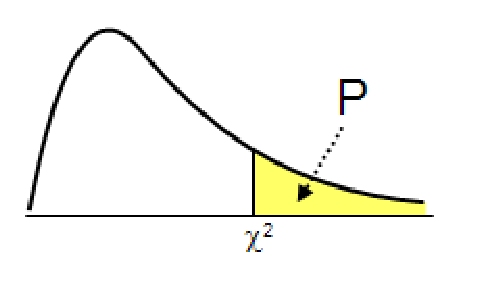
\includegraphics[scale=0.75]{chi}
							\tiny{
								\url{http://www.medcalc.org/manual/_help/images/chi-sq_curve.png}
							}
					\end{figure}
				\end{center}
			\end{frame}
		\end{center}

\section{Computational properties}
	\begin{frame}
		\begin{center}
			\begin{huge}
				Computational properties
			\end{huge}
		\end{center}
	\end{frame}
	\subsection{The MMHC}
		\begin{frame}
			\begin{block}{Remark to MMHC}
				\begin{itemize}
					\item  A hybrid algorithm \pause
					\begin{itemize}
						\item  Greedy Algorithm \pause
						\item  Constrained-based \pause
					\end{itemize}
					\item  np-hard
				\end{itemize} 
			\end{block}
		\end{frame}

\section{Example}
	\subsection{A practical example}
		\begin{frame}
				$
					\psmatrix[colsep=0.5cm,rowsep=0.5cm,mnode=circle]
					1&Difficulty&&Intelligence&2\\
					&3&Grade&&SAT\\
					&&Letter&4 \\
					&&5
					\ncline{->}{1,2}{2,3}
					\ncline{->}{1,4}{2,3}
					\ncline{->}{1,4}{2,5}
					\ncline{->}{2,3}{3,3}
					\endpsmatrix
				$
		\end{frame}

\section{Abschnitt Nr.3} 
\subsection{Tabellen}
\begin{frame}\frametitle{Tabellen}
	\begin{tabular}{|c|c|}
	\hline
	$\textbf{d}^{0}$ & $\textbf{d}^{1}$ \\
	\hline
	0.6 & 0.4  \\
	\hline
	\end{tabular}
\end{frame}

\section{Abschnitt Nr.3} 
\subsection{Tabellen}
\begin{frame}\frametitle{Tabellen}
	\begin{tabular}{|c|c|}
	\hline
	$\textbf{i}^{0}$ & $\textbf{i}^{1}$ \\
	\hline
	0.7 & 0.3  \\
	\hline
	\end{tabular}
\end{frame}

\section{Abschnitt Nr.3} 
\subsection{Tabellen}
\begin{frame}\frametitle{Tabellen}
	\begin{tabular}{|c|c|c|}
	\hline
	& $\textbf{s}^{0}$ & $\textbf{s}^{1}$ \\
	\hline
	$\textbf{i}^{0}$ & 0.95 & 0.05  \\
	\hline
	$\textbf{i}^{1}$ & 0.2 & 0.8  \\
	\hline
	\end{tabular}
\end{frame}

\section{Abschnitt Nr.3} 
\subsection{Tabellen}
\begin{frame}\frametitle{Tabellen}
	\begin{tabular}{|c|c|c|}
	\hline
	& $\textbf{l}^{0}$ & $\textbf{l}^{1}$ \\
	\hline
	$\textbf{g}^{1}$ & 0.95 & 0.05  \\
	\hline
	$\textbf{g}^{2}$ & 0.2 & 0.8  \\
	\hline
	$\textbf{g}^{3}$ & 0.2 & 0.8  \\
	\hline
	\end{tabular}
\end{frame}

\section{Abschnitt Nr.3} 
\subsection{Tabellen}
\begin{frame}\frametitle{Tabellen}
	\begin{tabular}{|c|c|c|c|}
	\hline
	& $\textbf{g}^{1}$ & $\textbf{g}^{2}$ & $\textbf{g}^{3}$ \\
	\hline
	$\textbf{i}^{0}$,$\textbf{d}^{0}$ & 0.3 & 0.4 & 0.3  \\
	\hline
	$\textbf{i}^{0}$,$\textbf{d}^{1}$ & 0.05 & 0.25 & 0.7  \\
	\hline
	$\textbf{i}^{1}$,$\textbf{d}^{0}$ & 0.9 & 0.08 & 0.02  \\
	\hline
	$\textbf{i}^{1}$,$\textbf{d}^{1}$ & 0.5 & 0.3 & 0.2  \\
	\hline
	\end{tabular}
\end{frame}

% \section{Abschnitt Nr. 5}
% \subsection{Geteilter Bildschirm}

% \begin{frame}\frametitle{Zerteilen des Bildschirmes}
% \begin{columns}
% \begin{column}{5cm}
% \begin{itemize}
% \item Beamer 
% \item Beamer Class 
% \item Beamer Class Latex 
% \end{itemize}
% \end{column}
% \begin{column}{5cm}
% \begin{tabular}{|c|c|}
% \hline
% \textbf{Kursleiter} & \textbf{Titel} \\
% \hline
% Sascha Frank &  \LaTeX \ Kurs 1 \\
% \hline
% Sascha Frank & \LaTeX \ Kursreihe \\
% \hline
% \end{tabular}
% \end{column}
% \end{columns}
% \end{frame}

\end{document}